\documentclass[Thesis.tex]{subfiles}
\begin{document}

\chapter{Introduction}

\begin{figure}
\centering
\resizebox{\textwidth}{!}{
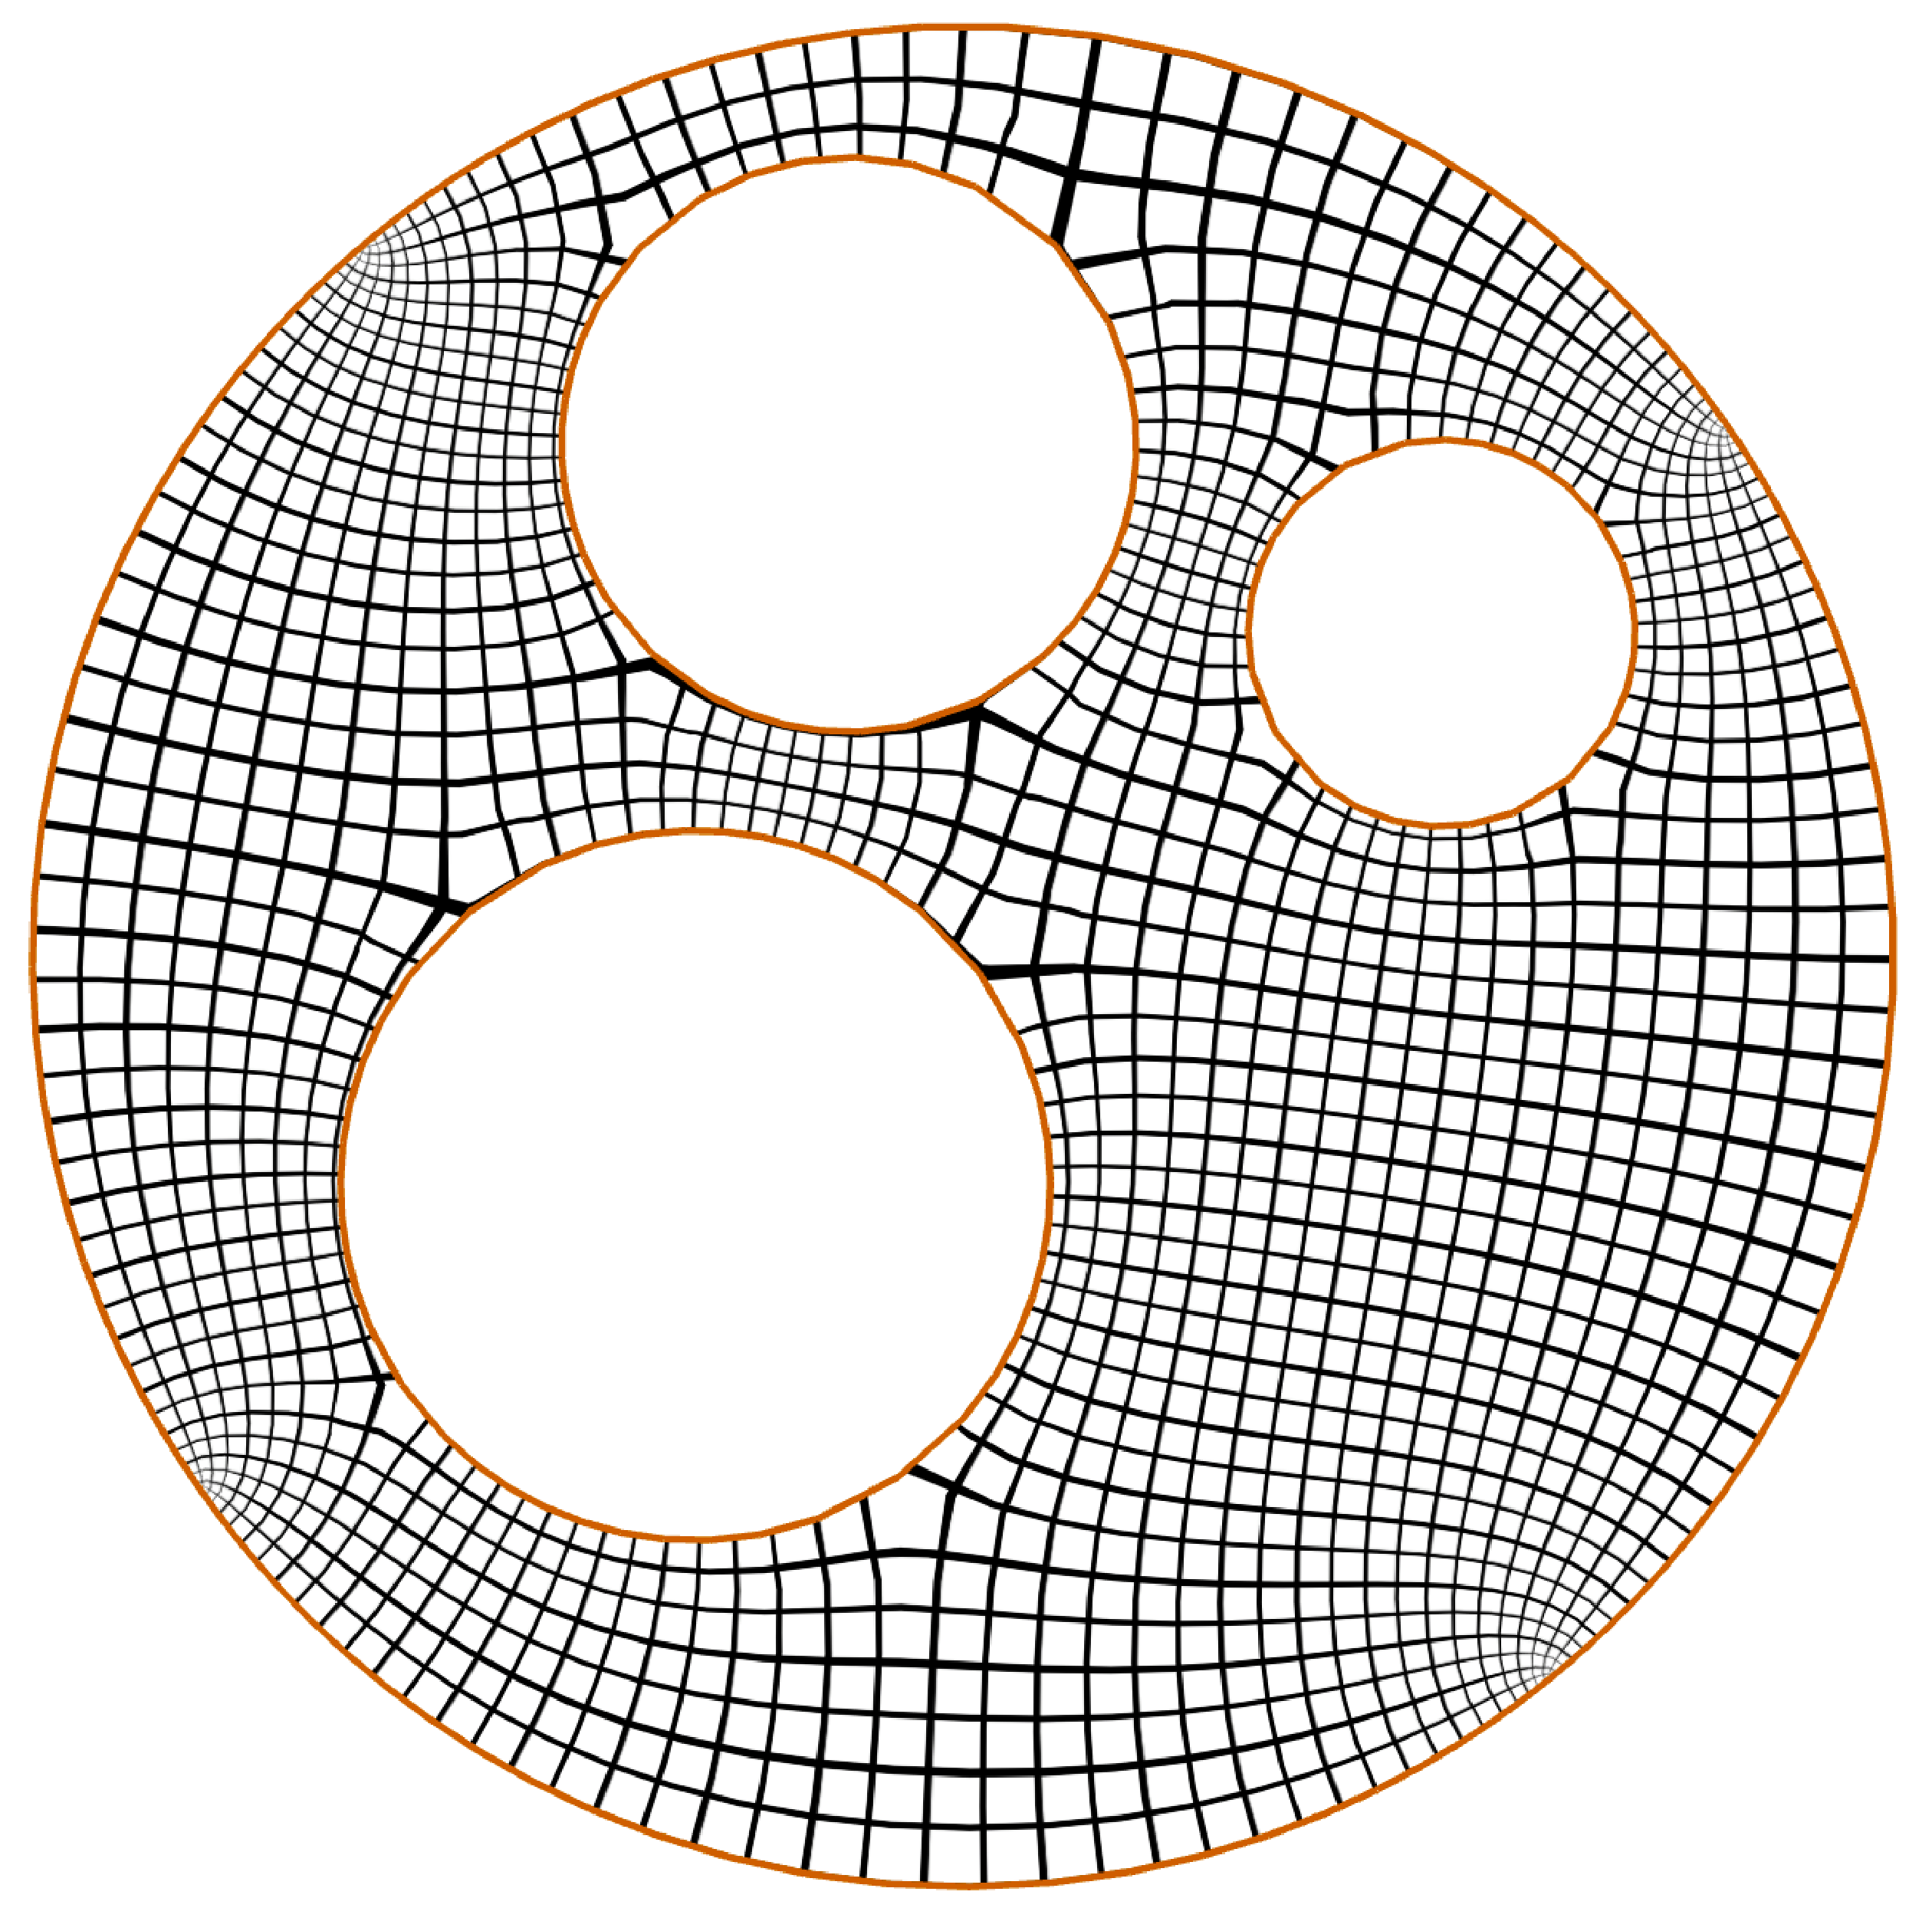
\includegraphics[height=4.8cm]{circle_domain_euclidean/three_holes_map.pdf}
\raisebox{0.25cm}{
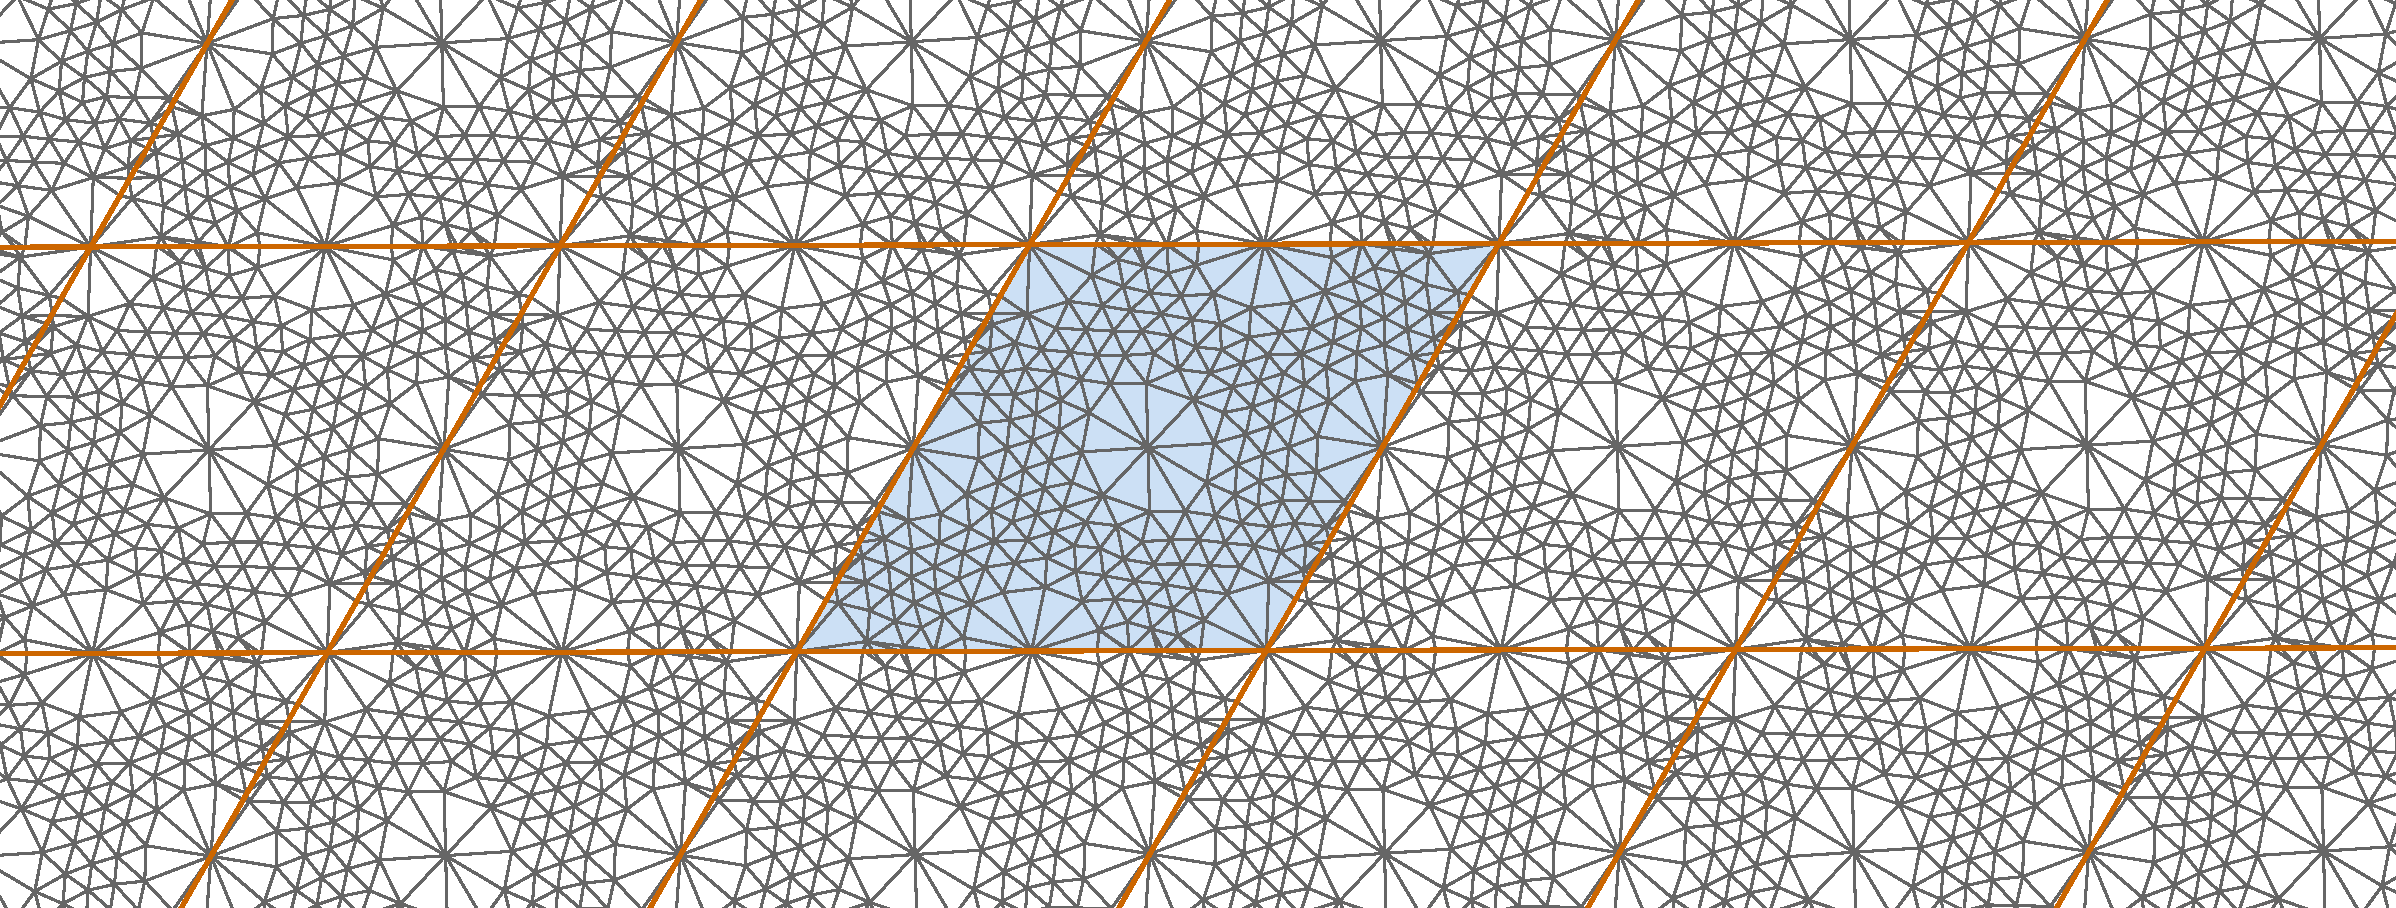
\includegraphics[height=4.5cm]{elliptic_curves/tetrahedron.pdf}
}
\includegraphics[height=5cm]{data/hyperelliptic_g3/cover_mesh}
}
\caption{
Discrete uniformizations of Riemann surfaces. 
Left: Region with four boundary components is mapped conformally to a domain bounded by circles, see Section~\ref{sec:circle_domains}. 
Middle: Uniformization of a discrete version of an elliptic curve. The image is a flat torus, see Section~\ref{sec:discrete_algebraic_curves}. 
Right: Uniformization of a hyperelliptic algebraic curve with a regular fundamental domain, see Section~\ref{sec:hyperelliptic}.
}
\label{fig:intro_uniformizations} 
\end{figure}

The notion of discrete conformal equivalence of triangle meshes was introduced in \cite{Springborn2008} and extended to hyperbolic metrics in \cite{Bobenko2010}. 
Two combinatorially equivalent euclidean triangle meshes are conformally equivalent if there exist scale factors associated to vertices such that corresponding edge lengths are equal up to multiplication with adjacent scale factors.
The problem of finding a discrete conformal map from a triangulated surface to the plane is formulated in terms of a variational principle using scale factors as variables.

Whereas the theoretical foundations of discrete conformal mappings via discrete conformal equivalence where arranged in the previous work, this thesis focuses of the experimental side of the theory. 
In the spirit of discrete differential geometry we look at theorems and constructions from the geometry of Riemann surfaces, e.g. embedded surfaces and their conformal structure, and find analogous discrete constructions with similar properties.
We investigate the generalization to cyclic polyhedral surfaces that was only touched upon in previous works.
We also give details on the spherical version of the theory that was put aside previously.

This thesis is divided into three parts. 

Part~I covers discrete uniformization of Riemann surfaces via conformal equivalence of cyclic polyhedral surfaces.
We generalize the variational principles established in \cite{Bobenko2010} and present a wealth of constructions and examples. 
Taken from smooth differential geometry and translated to the discrete setting we observe properties known from classic theorems. 
This culminates in a new conjecture about hyperelliptic Riemann surfaces. 
A Riemann surface is hyperelliptic if and only if the axes of the uniformization group elements meet in a common point for a suitable basis of the group, see Figure~\ref{fig:intro_uniformizations} right.
The tools created in the development of the methods used in this part lay the foundations for the applications presented in the Applications part.

\begin{figure}
\centering
\resizebox{\textwidth}{!}{
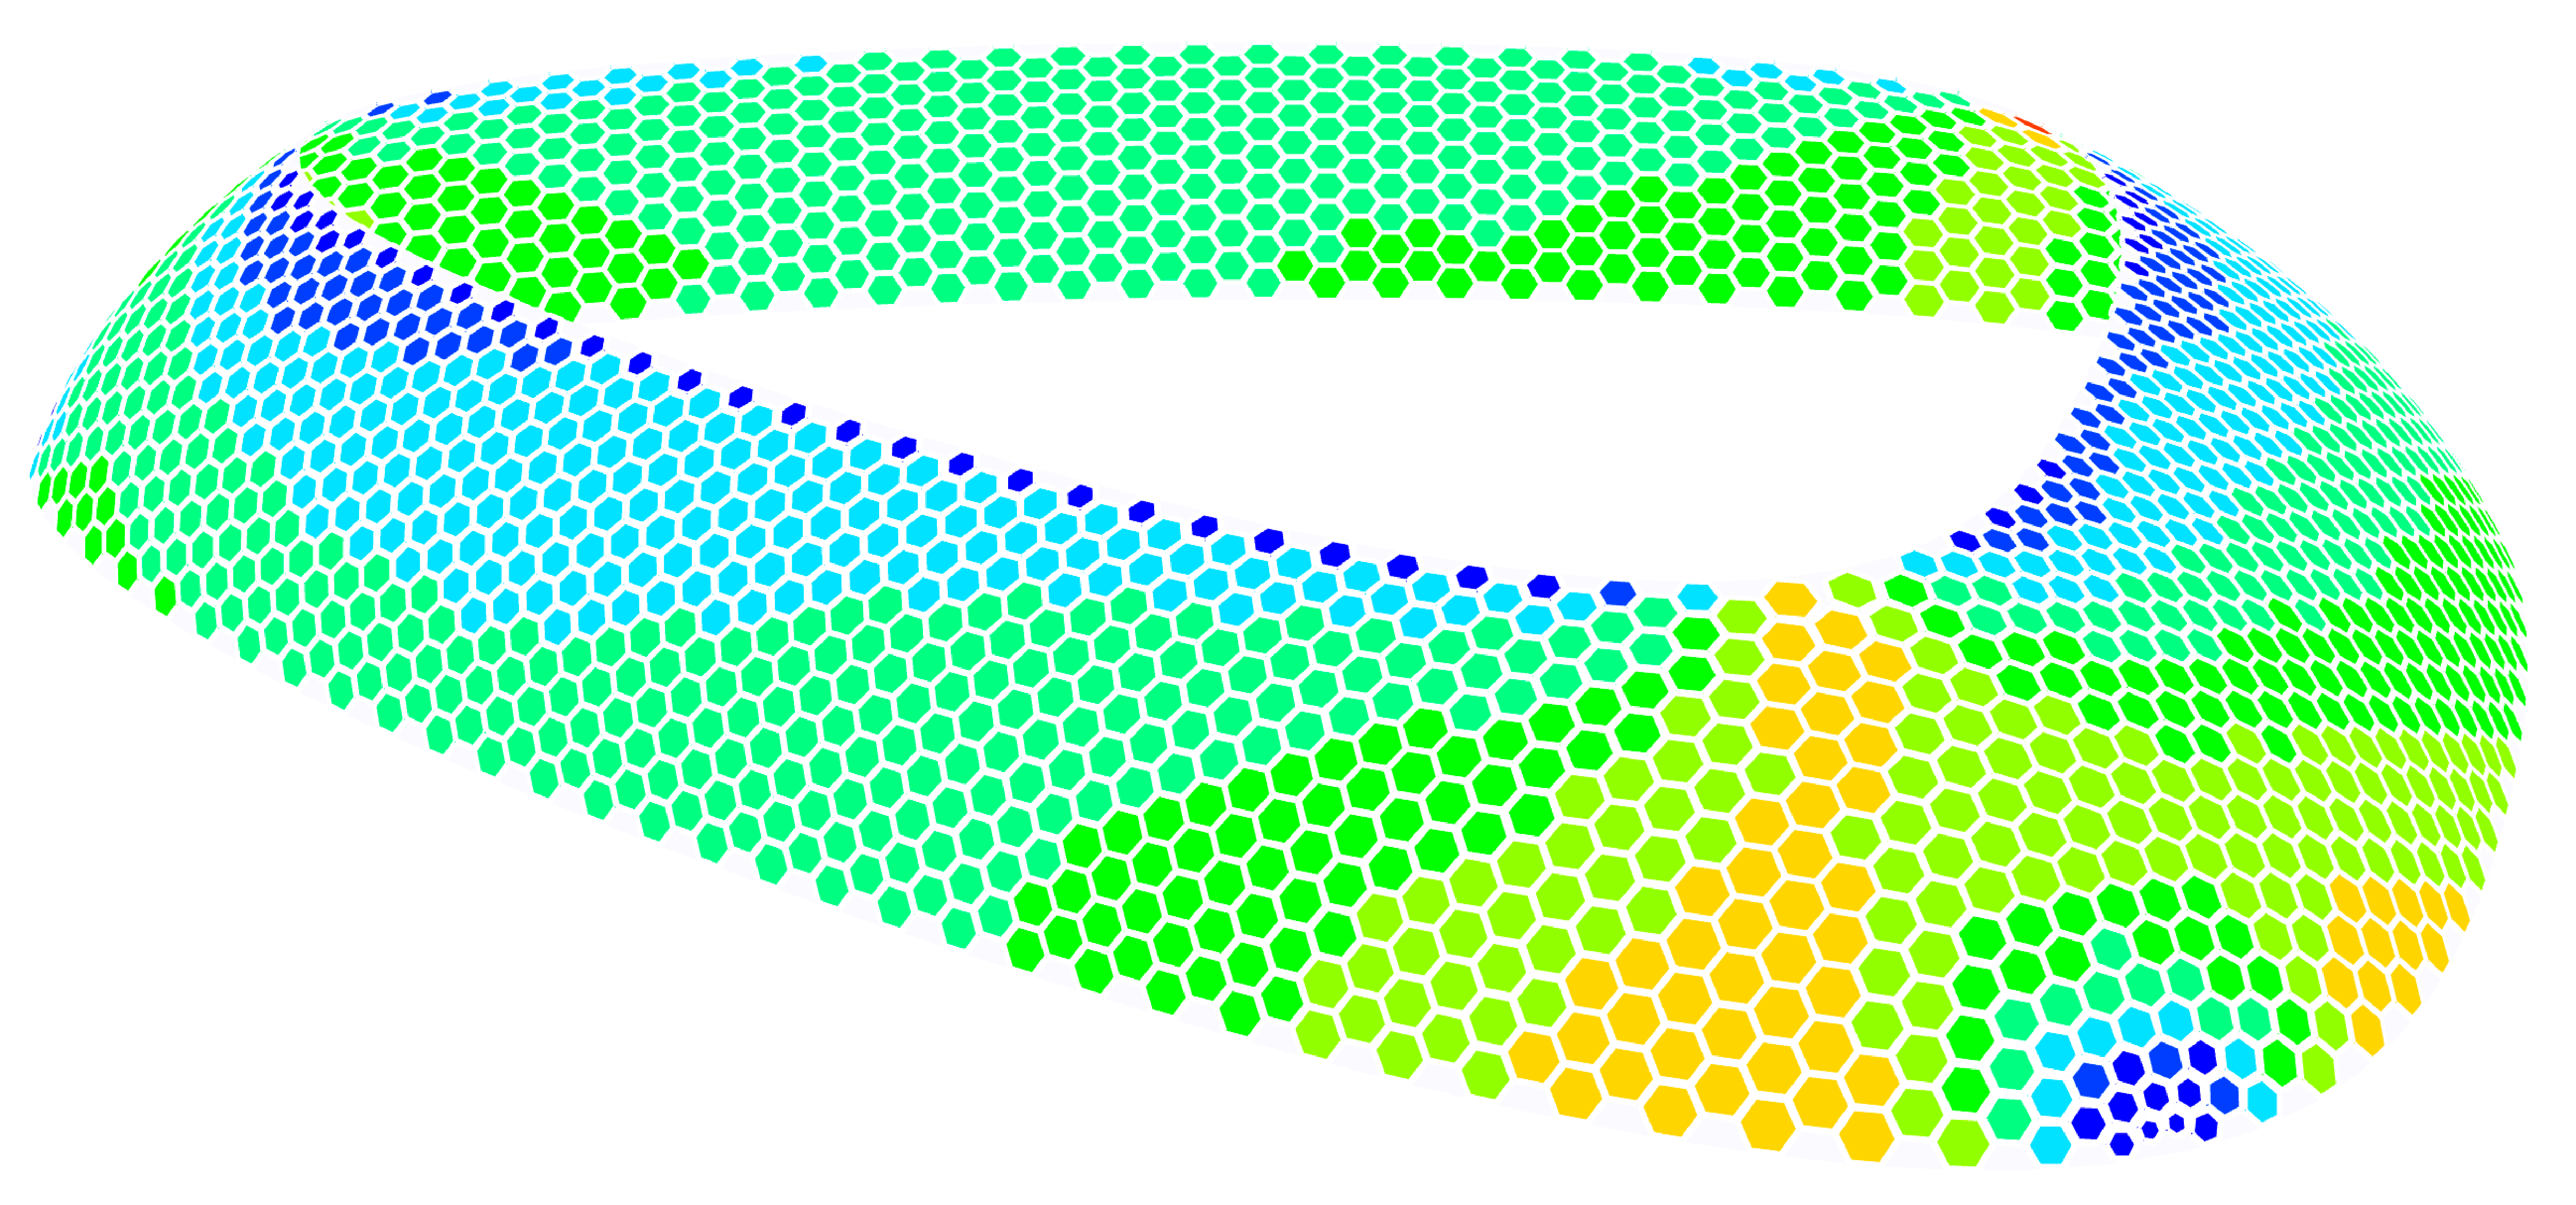
\includegraphics[height=4cm]{images/quantized_singularities5.pdf}
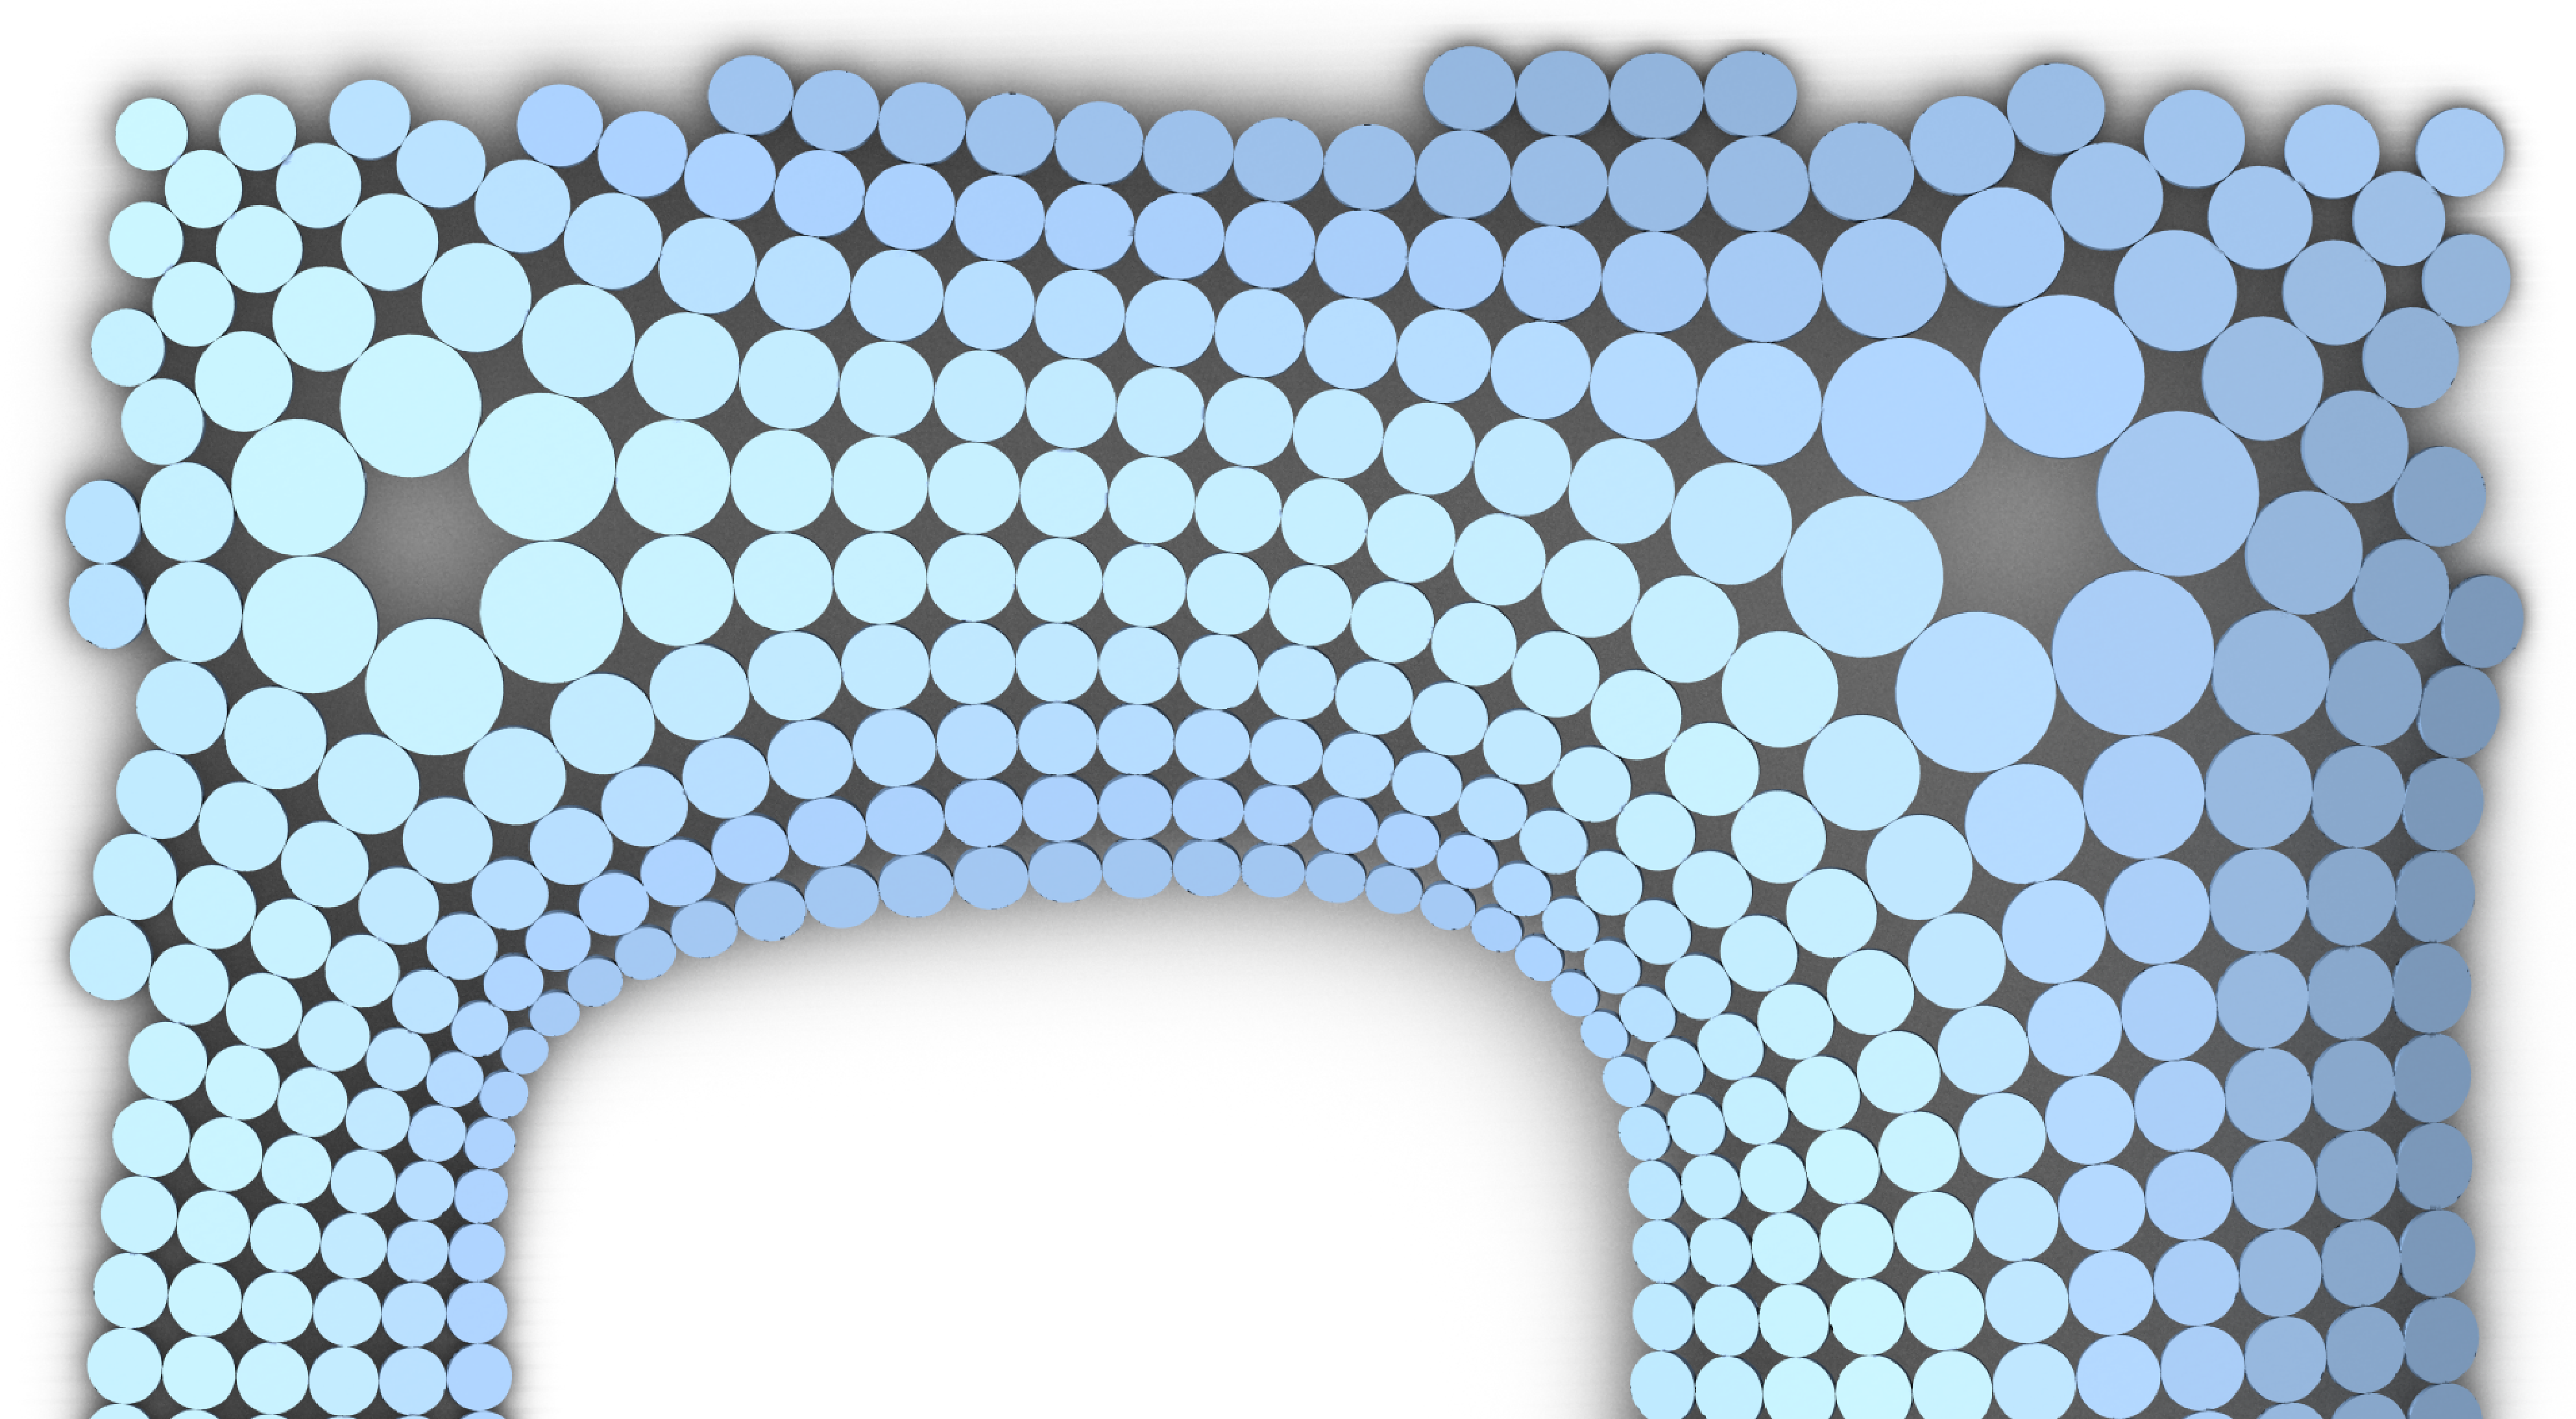
\includegraphics[height=4cm]{image/aag2012/dach_example01_circles.pdf}
}
\caption{
Two architectural applications of discrete conformal mappings. 
Left: A panel layout on a facade structure with size-quantized regular hexagons, see Chapter~\ref{chp:periodic_conformal_maps}.
Right: A circle pattern on a roof structure. 
We calculate discrete s-isothermic parameterizations for surfaces that are close to isothermic.
The resulting meshes exhibit planar faces. 
The mesh layout follows the directions of principle curvature, see Chapter~\ref{chp:quasiisothermic}.
}
\label{fig:intro_applications} 
\end{figure}

In Part~\ref{part:applications} we present three applications of discrete conformal mappings in the context of architectural geometry. 
In Chapter~\ref{chp:periodic_conformal_maps} we calculate regular patterns on architectural facade geometries with a period. 
We investigate how different boundary conditions affect the local behavior of the map.
The resulting map is used to create new meshes with regular faces such as hexagons.
We show how these meshes can be optimized towards a facade panel layout that can be fabricated in an efficient manner, see Figure~\ref{fig:intro_applications} left.

In Chapter~\ref{chp:quasiisothermic} we exploit the fact that isothermic surfaces possess a unique conformal curvature line parametrization to create meshes with planar quadrilaterals and touching incircles. 
This problem is formulated as a boundary value problem. 

In Chapter~\ref{chp:gridshells} we use discrete conformal maps as initialization for discrete Tschebyshev meshes, i.e., meshes with equal edges length. 
Starting from a discrete conformal map we perform non-linear optimization on quadrilateral meshes.
In doing so we control the curvature and intersection angles of parameter curves in the resulting gridshell construction.

The third part of this work introduces the reader to the software framework build for calculation with discrete surfaces and in particular with discrete conformal mappings, see Chapter~\ref{chp:conformallab}  about {\sc ConformalLab}, and discrete surface optimization, Chapter~\ref{chp:varylab} about {\sc VaryLab}. The author has implemented the software packages {\sc HalfEdge} and {\sc HalfEdgeTools}, see Chapter~\ref{chp:halfedge}, designed as a general tool for the calculation with discrete surfaces. Together with the user interface library {\sc JRWorkspace}, Chapter~\ref{chp:jrworkspace}, it constitutes a flexible framework for the creation of research applications in the context of discrete differential geometry. 

The digital data accompanying this work includes most of the examples presented in Chapter~\ref{chp:uniformization} and the main files for the architectural applications. Additionally we include the current state of the source code of the programming framework presented in Part~\ref{part:implementation}. The organization of the data is presented in the appendix.

\section*{Deutsche \"{U}bersetzung}
Diskrete konforme \"{A}quivalenz von Dreiecksnetzen wurde in \cite{Springborn2008} behandelt und in \cite{Bobenko2010} auf hyperbolische Metriken erweitert.
Zwei euklidische Triangulierungen mit gleicher Konnektivit\"{a}t sind diskret konform \"{a}quivalent, wenn es  Faktoren pro Ecke gibt, so dass entsprechende Kanten bis auf Multiplikation mit den Faktoren die gleiche L\"{a}nge haben.
Die konforme Abbildung von Triangulierten Fl\"{a}chen auf ebene Gebiete ist mit Hilfe eines Variationsprinzips auf den Skalierungsfaktoren formuliert.

Wir konzentrieren uns in dieser Abhandlung auf die experimentellen Aspekte der Theorie und st\"{u}tzen uns dabei auf die theoretischen Grundlagen aus den genannten Arbeiten.
Ganz im Geiste der diskreten Differentialgeometrie untersuchen wir Aussagen und Konstruktionen aus der Differentialgeometrie von glatten Fl\"{a}chen und versuchen diese in den diskreten Strukturen wieder zu finden.

Diese Abhandlung ist in drei Teile aufgeteilt, wovon der erste die konformen Abbildungen behandelt, der andere Anwendungen der Selbigen in der Architektur enth\"{a}lt und der dritte die Implementation der verwendeten Methoden in einer Software beschreibt.

Im ersten Teil beschreiben wir die diskrete Uniformisierung von Riemannschen Fl\"{a}chen mittels diskret konformer \"{A}quivalenz von zyklisch polyedrischen Fl\"{a}chen.
Wir verallgemeinern daf\"{u}r die bekannte Theorie der diskret konformen Dreiecksnetze auf zyklisch polyedrische Fl\"{a}chen.
Dieser Teil der Theorie wurde in vorangegangenen Arbeiten nur kurz ber\"{u}hrt.
Weiter beleuchten wir den sph\"{a}rischen Teil der Theorie, welcher bisher nicht behandelt worden ist.
Dieser Teil enth\"{a}lt auch eine neue Vermutung \"{u}ber hyperelliptische Riemannsche Fl\"{a}chen: 
Eine Riemannsche Fl\"{a}che ist hyperelliptisch genau dann, wenn es eine Basis der Uniformisierungsgruppe gibt, deren hyperbolische Achsen sich in einem gemeinsamen Punkt schneiden, siehe auch Abbildung~\ref{fig:intro_uniformizations} rechts.
Die Methoden aus diesem Abschnitt bilden die Grundlage f\"{u}r die Anwendungen in Teil~\ref{part:applications}.

Der zweite Teil enth\"{a}lt Anwendungen von konformen Abbildungen f\"{u}r die Architektur.
In Kapitel~\ref{chp:periodic_conformal_maps} werden regul\"{a}re Muster auf architektonischen Fassaden berechnet.
Daf\"{u}r verwenden wir periodische diskret konforme Abbildungen.
Wir untersuchen wie Randbedingungen das lokale Verhalten der Abbildungen beeinflussen.
Am Ende verwenden wir diese Abbildungen um die Geometrie von regul\"{a}ren Paneelen, zum Beispiel Sechsecken, zu bestimmen. 
Wir beschreiben wie diese Netze weiter optimiert werden um die Paneele effizient zu produzieren, siehe auch Abbildung~\ref{fig:intro_applications} links.

In Kapitel~\ref{chp:quasiisothermic} nutzen wir die Tatsache aus, dass Isothermfl\"{a}chen eindeutig nach Kr\"{u}mmungslinien parameterisierbar sind.
Wir berechnen s-isotherme Netze auf architektonischen Fl\"{a}chen, das sind Netze, deren ebene Facetten "sich an den Kanten ber\"{u}hrende" Kreise besitzen.
Dieses Problem ist als Randwertproblem von diskret konformen Abbildungen formuliert.

Kapitel~\ref{chp:gridshells} gibt eine Einf\"{u}hrung in das Konzept der architektonischen Gitterschalen.
Geometrisch sind das Netze mit gleich langen Kanten.
Ausgehend von diskret konformen Abbildungen berechnen wir diese Strukturen mittels nicht-linearer Optimierung von Vierecksnetzen.

Der dritte Teil f\"{u}hrt den Leser in das Software-Framework ein, welches f\"{u}r Berechnungen an diskreten Fl\"{a}chen und speziell konformen Abbildungen entworfen wurde, siehe hierf\"{u}r Kapitel~\ref{chp:conformallab} \"{u}ber {\sc ConformalLab}.
Der Teil, der sich mit Optimierung von diskreten Fl\"{a}chen besch\"{a}ftigt ist, im Kapitel~\ref{chp:varylab} \"{u}ber {\sc VaryLab} beschrieben.

Der Autor hat weiter die Bibliotheken {\sc HalfEdge} and {\sc HalfEdgeTools} entworfen, siehe Kapitel~\ref{chp:halfedge}.
Diese sind als allgemeine Werkzeuge f\"ur Berechnungen an diskreten F\"{a}chen entworfen.
Zusammen mit der Oberfl\"{a}chenbibliothek {\sc JRWorkspace}, Kapitel~\ref{chp:jrworkspace}, bilden sie ein flexibles Framework f\"{u}r den Entwurf komplexer Forschungsanwendungen im Bereich der diskreten Differentialgeometrie.

Diese Arbeit enth\"{a}lt eine CD mit digitalen den Daten der meisten Beispiele aus Kapitel~\ref{chp:uniformization} und den architektonischen Anwendungen.
Zus\"{a}tzlich ist der Quellcode der in Teil~\ref{part:implementation} beschriebenen Software in seiner aktuellen Fassung sowie einer kompilierten lauff\"{a}higen Version enthalten.
Die Struktur dieser Daten ist im Anhang beschrieben.

\subfilebibliography
\end{document}

%%% Local Variables:
%%% TeX-master: "Thesis.tex"
%%% End: